\chapter{Kết quả \& Thảo luận}
\label{Chapter5}

\section{Huấn luyện tập trung \& thuật toán $FedAvg$}

% trình bày huấn luyện tập trung với fedAvg iid

Dựa theo định nghĩa về một hệ thống FL, với cùng một kiến trúc mô hình, khoá luận tiến hành so sánh kết quả của quá trình huấn luyện tập trung và huấn luyện phân tán (thuật toán \codeword{FedAvg} trên các kịch bản dữ liệu IID và Non-IID). Kết quả được trình bày trong Bảng \ref{fig:central_decentral}.

\begin{table}[H]
    \centering
    \caption{Kết quả (\%) huấn luyện tập trung và thuật toán FedAvg (IID và Non-IID) trên MNIST và CIFAR-10}
    \label{fig:central_decentral}
    \resizebox{\linewidth}{!}{%
    \begin{tabular}{c|l|ccccc} 
    \toprule
    \multicolumn{1}{c}{}      &                                & $acc_{micro}$    & $acc_{macro}$ & $P_{macro}$      & $R_{macro}$      & $F1_{macro}$      \\ 
    \hline
    \multirow{4}{*}{MNIST}    & Centralized                    & \textbf{97.07} & -           & \textbf{97.04} & \textbf{97.03} & \textbf{97.04}  \\
                              & FedAvg (IID data)                   & 90.36          & 90.34±2.24  & 90.37±2.29     & 90.25±2.22     & 90.12±2.29      \\
                              & FedAvg (local client) & 85.03          & 82.14±14.76 & 82.03±13.88    & 81.54±14.33    & 79.43±16.83     \\
                              & FedAvg (new client)   & 83.92          & 81.69±19.71 & 79.57±20.18    & 80.46±17.84    & 77.66±22.54     \\ 
    \hline
    \multirow{4}{*}{CIFAR-10} & Centralized                    & \textbf{61.91} & -           & \textbf{61.7}  & \textbf{62.01} & \textbf{61.72}  \\
                              & FedAvg (IID data)                   & 53.83          & 53.83±3.14  & 53.46±3.19     & 53.85±3.26     & 53±3.21         \\
                              & FedAvg (local client) & 19.02          & 19.29±25.11 & 15.57±23.7     & 20.65±25.55    & 16.85±23.92     \\
                              & FedAvg (new client)   & 24.63          & 24.83±22.57 & 18.36±20.15    & 24.44±21.95    & 20.52±20.45     \\
    \bottomrule
    \end{tabular}
    }
\end{table}

Dễ dàng nhận thấy, mô hình huấn luyện tập trung đạt kết quả cao hơn trên tất cả các thang đánh giá (trừ $acc_{macro}$, vì huấn luyện tập trung không bao gồm bất kỳ người dùng nào nên không thể lấy trung bình cộng kết quả của từng người dùng). Dữ liệu huấn luyện tập trung tuân theo phân phối đều nên sự phân lớp của mô hình không thiên về bất cứ lớp dữ liệu nào, dẫn đến các kết quả thu được có giá trị xấp xỉ nhau (chênh lệch dưới 1\%).

Các kết quả thu được trên \codeword{FedAvg} (dữ liệu IID) thấp hơn từ 7\% đến 8\% do mô hình toàn cục nắm bắt các đặc trưng một cách gián tiếp (thông qua quá trình lấy trung bình tham số tại máy chủ). Các giá trị này cũng khá đều nhau (chênh lệch dưới 1\%) trên từng tập dữ liệu do việc sử dụng dữ liệu IID trong huấn luyện phân tán.

Thuật toán \codeword{FedAvg} do Google đề xuất được giới thiệu về khả năng "chống chịu" tốt trên dữ liệu Non-IID \cite{mcmahan2017communication}. Tuy nhiên, khoá luận này cùng nhiều nghiên cứu khác (\parencite{chen2018federated, wang2019federated, zhao2018federated, zhu2021federated}) không đồng ý với quan điểm này. Thật vậy, Bảng \ref{fig:central_decentral} cho thấy các giá trị độ đo giảm từ 9\% đến 13\% trên MNIST và không đạt hội tụ trên CIFAR-10 khi dữ liệu đầu vào của hệ thống FL chuyển từ IID sang Non-IID. Các giá trị độ đo trên dữ liệu Non-IID cũng chênh lệch nhau khá nhiều (2\% - 8\% trên MNIST và 1\% - 6\% trên CIFAR-10) so với chênh lệch trên dữ liệu IID (dưới 1\%). Điều này chứng tỏ phân phối dữ liệu không đều trên các máy khách đã ảnh hưởng xấu đến chất lượng phân lớp.

Về mặt lý thuyết, hiện tượng giảm hiệu suất trên dữ liệu Non-IID là do mô hình toàn cục không được huấn luyện trên một phân phối đều nên ước lượng đạo hàm trên từng batch dữ liệu không đại diện được cho đạo hàm trên toàn bộ dữ liệu. Trong quá trình kiểm thử, khi đứng trước một phân phối dữ liệu lạ, mô hình toàn cục không thể nào nắm bắt được đặc trưng dữ liệu một cách hiệu quả dẫn đến việc phân lớp không chính xác. Một cách dễ hiểu, dữ liệu kiểm thử trên các máy khách có tính cá nhân hóa cao và rất khác với những gì mô hình đã được huấn luyện trước đó nên mô hình hoạt động không tốt.

\section{Phân tích khả năng hội tụ}

% fedMeta-per vs fedAvg, FedAvgMeta, FedPer, FedPerMeta
% bêu xấu fedAvg, FedAvgMeta, FedPer, FedPerMeta đã đời (giải thích lý do)
% fedMeta-per xịn hơn là vì đâu?

Để giải quyết vấn đề dữ liệu Non-IID, kỹ thuật fine-tune cục bộ được thêm vào hệ thống FL dưới dạng đơn giản (thuật toán \codeword{FedAvgMeta}), nhằm cải thiện khả năng thích ứng của mô hình trên tập dữ liệu mới . Tuy nhiên, kết quả thu được không mấy khả quan. Giá trị các thang đo trên tập dữ liệu MNIST giảm khoảng 1\% khi kiểm thử trên người dùng cục bộ và tăng khoảng 1\% khi kiểm thử trên người dùng mới so với \codeword{FedAvg} (Bảng \ref{tab:mnist}). Trên tập dữ liệu CIFAR-10, mô hình vẫn tiếp tục không đạt hội tụ (Hình \ref{fig:cifar_meta_new} và \ref{fig:cifar_meta_old}). Nói chung, sau khi áp dụng kỹ thuật fine-tune cục bộ ở mức đơn giản, các kết quả thu được không thể hiện được sự cải thiện rõ rệt. Nguyên nhân cho việc này nằm ở chỗ khả năng thích ứng trên tập dữ liệu mới của mô hình toàn cục là rất thấp.

\begin{table}[H]
    \centering
    \caption{Bảng kết quả (\%) của thuật toán FedMeta và FedAvg trên tập dữ liệu MNIST}
    \label{tab:mnist}
    \resizebox{\linewidth}{!}{%
    \begin{tabular}{c|l|ccccc} 
    \toprule
    \multicolumn{1}{l}{}                             & \multicolumn{1}{c|}{} & $acc_{micro}$    & $acc_{macro}$          & $P_{macro}$            & $R_{macro}$            & $F1_{macro}$            \\ 
    \hline
    \multirow{4}{*}{local client}                    & FedAvg                & 85.03           & 82.14±14.76          & 82.03±13.88           & 81.54±14.33          & 79.43±16.83           \\
                                                     & FedAvgMeta            & 84.84           & 81.56±16.68          & 80.71±17.02           & 81.18±16.16          & 78.31±19.8            \\
                                                     & FedMeta(MAML)         & 92.99           & 91.14±5.99           & 90.56±6.24            & 90.98±5.9            & 90.16±6.28            \\
                                                     & FedMeta(Meta-SGD)     & \textbf{98.02 } & \textbf{96.35±4.62 } & \textbf{96.49±4.1 }   & \textbf{95.64±5.94 } & \textbf{95.80±5.51 }  \\ 
    \hline
    \multicolumn{1}{l|}{\multirow{4}{*}{new client}} & FedAvg                & 83.92           & 81.69±19.71          & 79.57±20.18           & 80.46±17.84          & 77.66±22.54           \\
    \multicolumn{1}{l|}{}                            & FedAvgMeta            & 84.34           & 82.37±17.42          & 81.38±16.25           & 80.91±15.62          & 78.78±19.31           \\
    \multicolumn{1}{l|}{}                            & FedMeta(MAML)         & 92.96           & 91.88±5.88           & 90.14±7.97            & \textbf{90.74±5.95 } & \textbf{90.02±7.34 }  \\
    \multicolumn{1}{l|}{}                            & FedMeta(Meta-SGD)     & \textbf{96.39 } & \textbf{93.53±8.39 } & \textbf{93.73±10.26 } & 88.65±14.06          & 89.31±14.56           \\
    \bottomrule
    \end{tabular}
    }
\end{table}

Kỹ thuật sử dụng lớp cá nhân hoá cũng được đưa vào giải quyết vấn đề dữ liệu Non-IID. Thuật toán được sử dụng trong khoá luận là \codeword{FedPer} và một phiên bản cho phép fine-tune trên tập support trong quá trình kiểm thử - \codeword{FedPerMeta}. Các lớp phần riêng tại đây được kỳ vọng sẽ nắm bắt thành công các đặc trưng của từng máy khách trong kịch bản dữ liệu Non-IID. Qua quan sát Hình \ref{fig:fedper_acc}, rõ ràng hai thuật toán trên đã không đạt được kỳ vọng này. Các kết quả thu được thậm chí còn tệ hơn thuật toán \codeword{FedAvg} và khả năng hội tụ của hai thuật toán này gần như tương đồng và đôi lúc có phần "đuối" hơn so với \codeword{FedAvg} trên tất cả các kịch bản kiểm thử.

Trong khi đó, Bảng \ref{tab:acc_paper} cho thấy độ chính xác của thuật toán \codeword{FedPer} đạt 83.39±0.47\% (hệ thống gồm 50 máy khách trên dữ liệu CIFAR-10 Non-IID). Điều này dễ dàng được giải thích khi kiến trúc mạng học sâu mà \codeword{FedPer} sử dụng để tạo ra kết quả trên là mạng pre-trained \codeword{MobileNet-v1} \cite{howard2017mobilenets}. Nhờ vào \codeword{MobileNet-v1}, một mạng học sâu phức tạp hơn kiến trúc sử dụng trong khoá luận rất nhiều lần, hệ thống FL rút trích được nhiều đặc trưng hơn và đạt kết quả tốt hơn. Tuy nhiên, chi phí phần cứng cho việc duy trì các lớp phần riêng tại máy khách cũng tăng lên. Trái lại, mạng học sâu mà khoá luận sử dụng rất đơn giản, giúp làm giảm đáng kể chi phí phần cứng nhưng hiệu quả đem lại rất cao (Hình \ref{fig:fedper_acc}).

Nhằm kiểm chứng khả năng thích ứng nhanh trên tập dữ liệu mới của ML, cũng như hiệu suất của hệ thống FL có tích hợp ML, khoá luận thí nghiệm trên các thuật toán \codeword{FedMeta} và thu được kết quả như Bảng \ref{tab:mnist} và \ref{tab:cifar}. Theo đó, ML giúp cải thiện 20\% đến 60\% trên tập CIFAR-10 và 11\% đến 16\% trên tập MNIST trên cả năm thang độ đo.

\begin{table}[H]
    \centering
    \caption{Bảng kết quả (\%) của thuật toán FedMeta và FedAvg trên tập dữ liệu CIFAR-10}
    \label{tab:cifar}
    \resizebox{\linewidth}{!}{%
    \begin{tabular}{c|l|ccccc} 
    \toprule
    \multicolumn{1}{l}{}                             & \multicolumn{1}{c|}{} & $acc_{micro}$    & $acc_{macro}$          & $P_{macro}$            & $R_{macro}$            & $F1_{macro}$            \\ 
    \hline
    \multirow{4}{*}{local client}                    & FedAvg                & 19.02          & 19.29±25.11          & 15.57±23.7           & 20.65±25.55          & 16.85±23.92           \\
                                                     & FedAvgMeta            & 40.3           & 38.47±31.52          & 32.84±32.06          & 39.33±30.35          & 33.81±30.61           \\
                                                     & FedMeta(MAML)         & 69.02          & 68.76±14.86          & 67.42±21.16          & 66.56±13.48          & 61.14±20              \\
                                                     & FedMeta(Meta-SGD)     & \textbf{78.63} & \textbf{78.73±11.59} & \textbf{74.65±21.12} & \textbf{75.25±14.09} & \textbf{72.87±18.31}  \\ 
    \hline
    \multicolumn{1}{l|}{\multirow{4}{*}{new client}} & FedAvg                & 24.63          & 24.83±22.57          & 18.36±20.15          & 24.44±21.95          & 20.52±20.45           \\
    \multicolumn{1}{l|}{}                            & FedAvgMeta            & 43.39          & 43.54±18             & 33.45±21.44          & 42.87±16.98          & 35.14±17.22           \\
    \multicolumn{1}{l|}{}                            & FedMeta(MAML)         & 61.69          & 61.64±12.49          & 52.66±26.06          & 59.94±12.35          & 50.76±19.2            \\
    \multicolumn{1}{l|}{}                            & FedMeta(Meta-SGD)     & \textbf{68.36} & \textbf{67.89±15.11} & \textbf{70.3±22.37}  & \textbf{66.86±15.02} & \textbf{60.24±21.52}  \\
    \bottomrule
    \end{tabular}
    }
\end{table}

Quan sát kỹ hơn quá trình hội tụ của các thuật toán \codeword{FedMeta} (Hình \ref{fig:fedmeta_acc}), có thể dễ dàng nhận thấy, thuật toán này hội tụ nhanh hơn và đạt độ chính xác cao hơn \codeword{FedAvg} và \codeword{FedAvgMeta}. Đối với tập dữ liệu CIFAR-10, chỉ trong vòng 25 bước (đối với người dùng mới) và 100 bước (đối với người dùng cục bộ) huấn luyện cục bộ đầu tiên, độ chính xác đạt được đã tiệm cận ngưỡng hội tụ trong khi \codeword{FedAvg} và \codeword{FedAvgMeta} không ổn định và không đạt hội tụ sau 600 bước huấn luyện. Tập dữ liệu MNIST với dữ liệu ảnh đen trắng khiến việc huấn luyện trở nên dễ dàng hơn: chỉ sau 50 bước huấn luyện (trên cả người dùng mói lẫn người dùng cục bộ), các thuật toán đã đều gần chạm ngưỡng hội tụ của mình. Tuy nhiên, mức hội tụ của các thuật toán \codeword{FedMeta} vẫn tỏ ra nổi trội khi bỏ xa hai thuật toán còn lại 20\% chỉ trong 50 bước huấn luyện đầu tiên.

Việc hội tụ này càng đặc biệt hơn khi mô hình toàn cục thể hiện sự thích ứng với tập dữ liệu mới rất nhanh bằng cách thi triển một bước huấn luyện trên 20\% dữ liệu kiểm tra tại máy khách. Điều này đã chứng minh được khả năng thích ứng nhanh trên tập dữ liệu mới của các thuật toán ML.

Từ Hình \ref{fig:fedmetaper_acc}, có thể thấy sự tương đồng về hình dạng đường hội tụ của \codeword{FedMeta-Per} và \codeword{FedMeta}, cũng như việc các thuật toán đề xuất đạt độ chính xác rất cao, đôi khi còn có phần nhỉnh hơn so với \codeword{FedMeta}. \textbf{Đây chính là bằng chứng, chứng minh việc thuật toán đề xuất đạt hội tụ nhanh chính nhờ vào khả năng thích ứng nhanh trên tập dữ liệu mới do ML cung cấp} chứ không đến từ bất kỳ nguyên nhân nào khác. Do đó, các kết quả thu được trong Hình \ref{fig:fedper_acc} là hoàn toàn dễ hiểu khi khả năng hội tụ của thuật toán đề xuất bỏ xa các thuật toán \codeword{FedAvg} và \codeword{FedPer}.

\begin{sidewaysfigure}
    \centering
    \begin{subfigure}{\textwidth}
        \centering
        \begin{subfigure}{.5\textwidth}
            \centering
            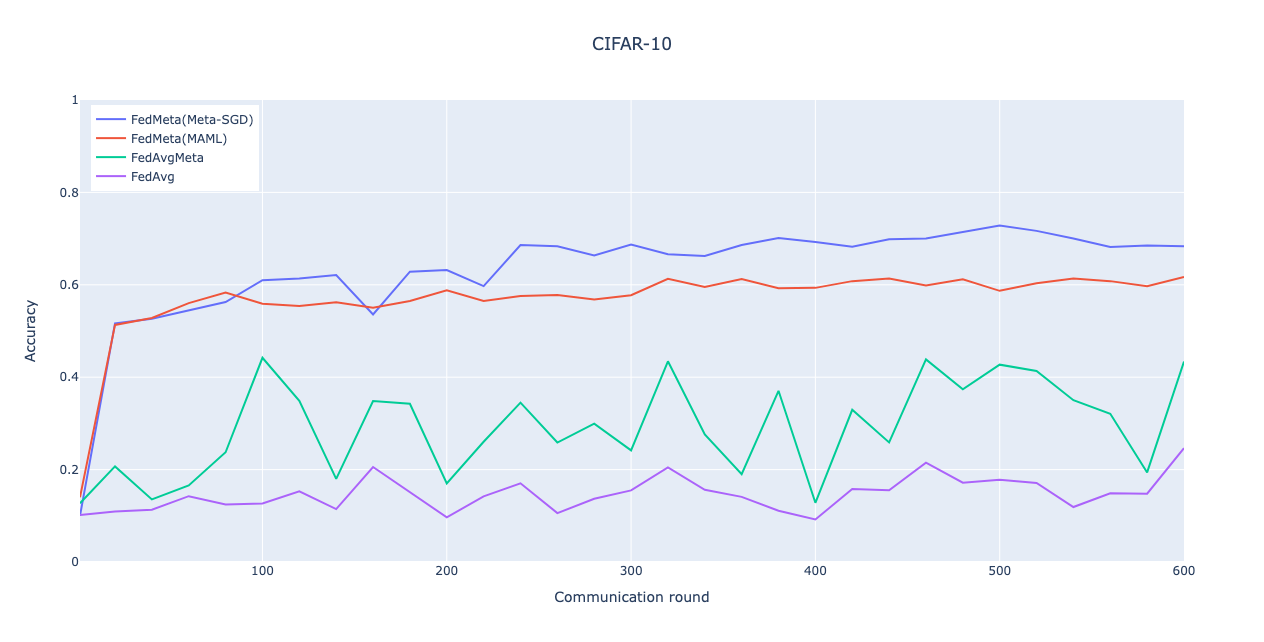
\includegraphics[width=\linewidth]{./images/cifar_meta_new.png}
            \caption{CIFAR-10, new clients}
            \label{fig:cifar_meta_new}
        \end{subfigure}%
        \begin{subfigure}{.5\textwidth}
            \centering
            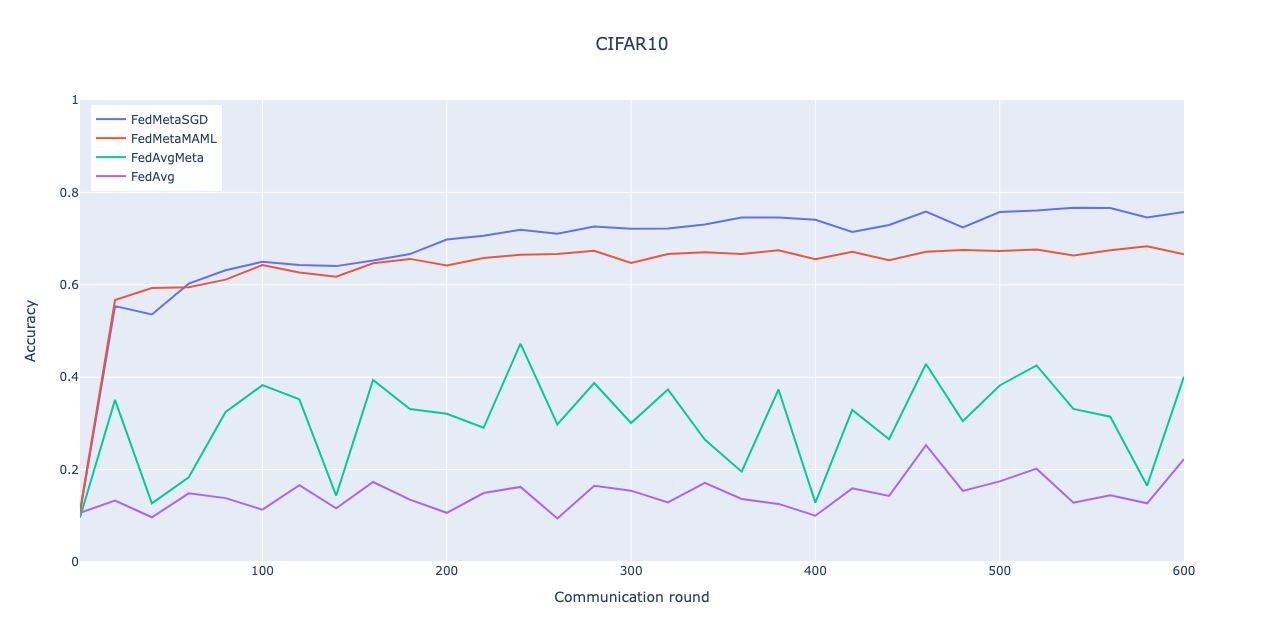
\includegraphics[width=\linewidth]{./images/cifar_meta_old.png}
            \caption{CIFAR-10, local clients}
            \label{fig:cifar_meta_old}
        \end{subfigure}
        % \caption{A figure with two subfigures}
        % \label{fig:test}
    \end{subfigure}

    \begin{subfigure}{\textwidth}
        \centering
        \begin{subfigure}{.5\textwidth}
            \centering
            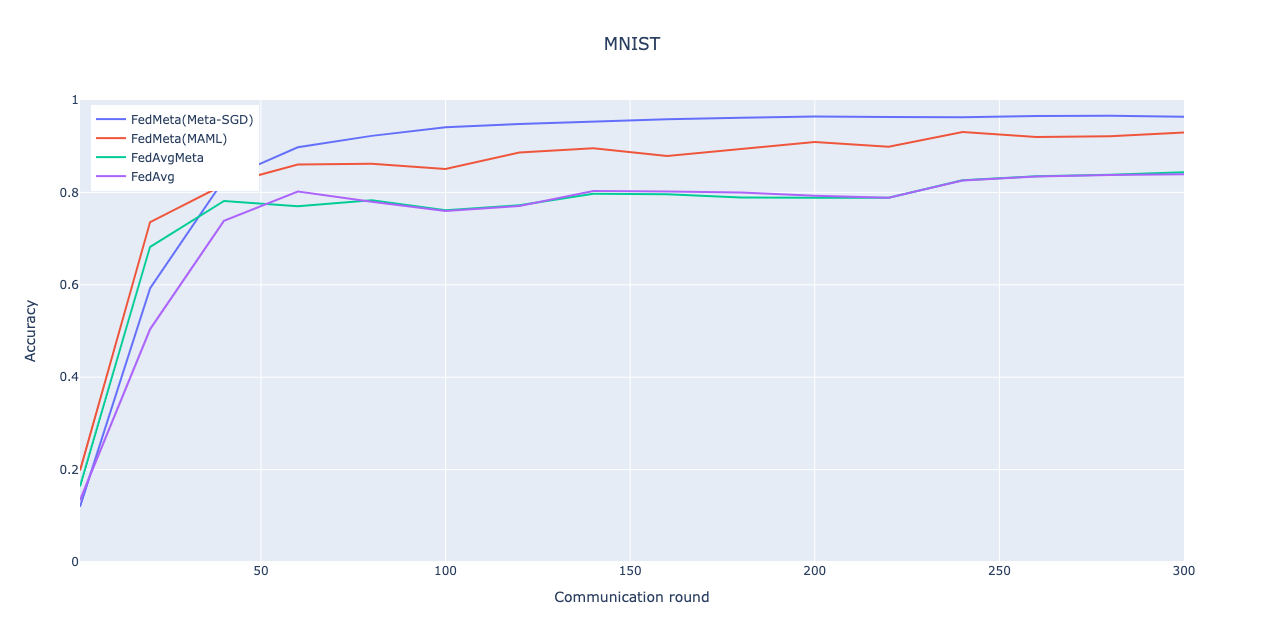
\includegraphics[width=\linewidth]{./images/mnist_meta_new.png}
            \caption{MNIST, new clients}
            \label{fig:mnist_meta_new}
        \end{subfigure}%
        \begin{subfigure}{.5\textwidth}
            \centering
            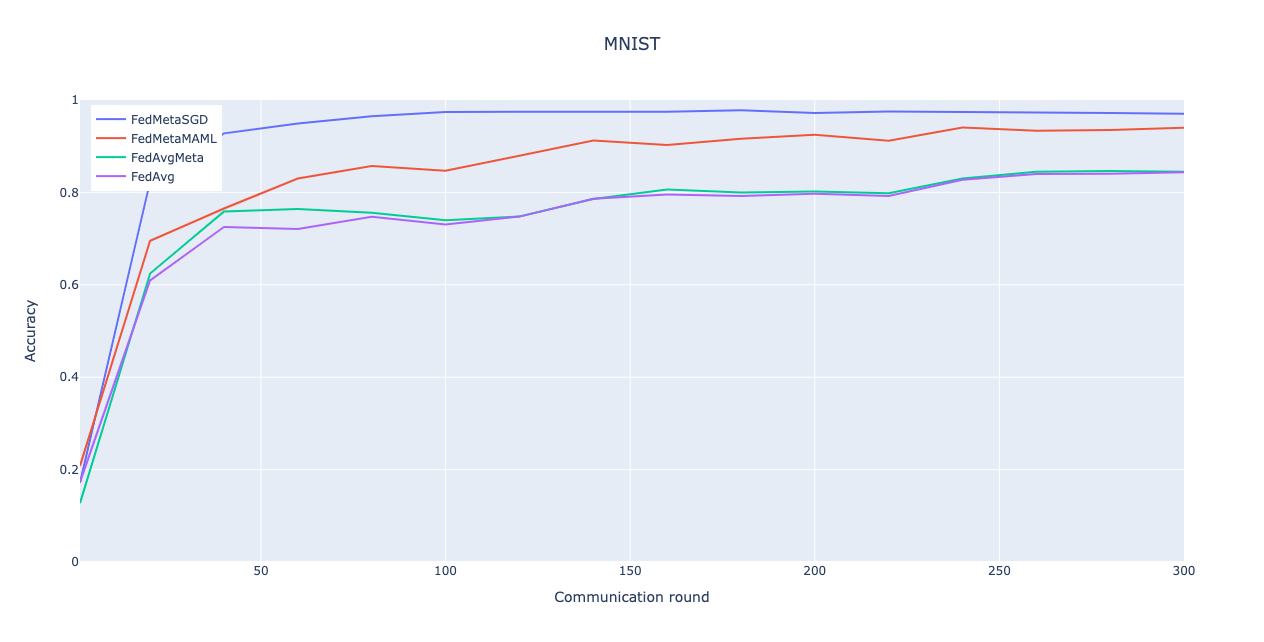
\includegraphics[width=\linewidth]{./images/mnist_meta_old.png}
            \caption{MNIST, local clients}
            \label{fig:mnist_meta_old}
        \end{subfigure}
        % \caption{A figure with two subfigures}
        % \label{fig:test}
    \end{subfigure}
    \caption{Quá trình hội tụ của FedAvg và FedMeta}
    \label{fig:fedmeta_acc}
\end{sidewaysfigure}

\begin{sidewaysfigure}
    \centering
    \begin{subfigure}{\textwidth}
        \centering
        \begin{subfigure}{.5\textwidth}
            \centering
            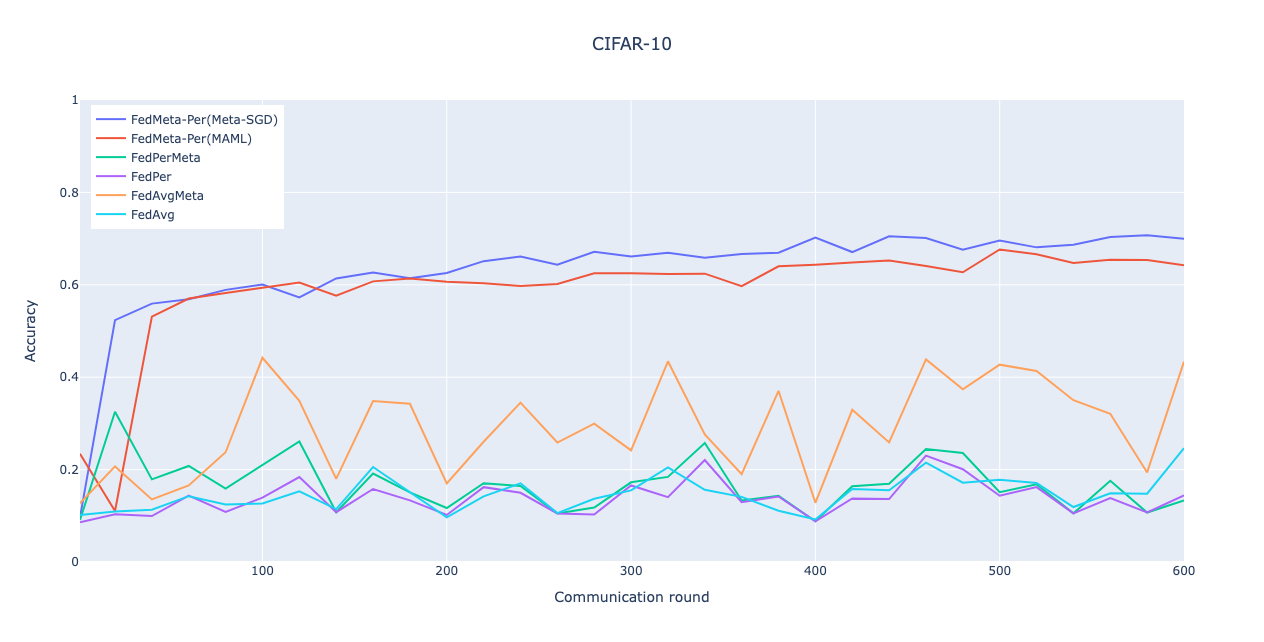
\includegraphics[width=\linewidth]{./tab_img/cifar_per_new.png}
            \caption{CIFAR-10, new clients}
            \label{fig:cifar_per_new}
        \end{subfigure}%
        \begin{subfigure}{.5\textwidth}
            \centering
            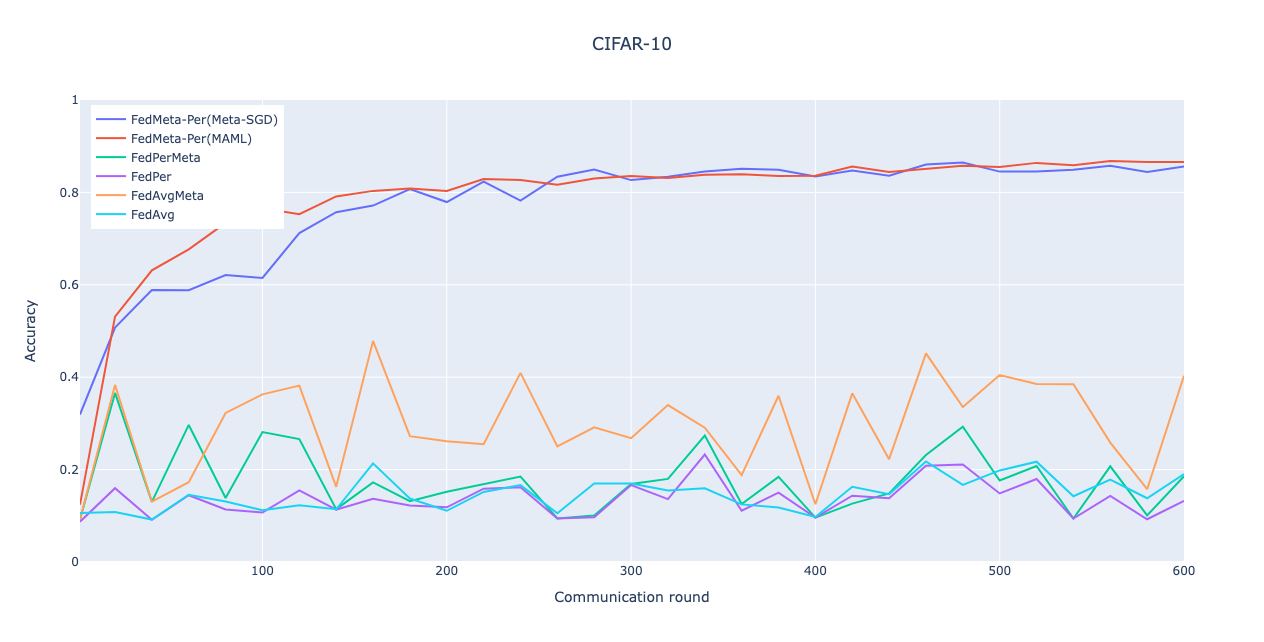
\includegraphics[width=\linewidth]{./tab_img/cifar_per_old.png}
            \caption{CIFAR-10, local clients}
            \label{fig:cifar_per_old}
        \end{subfigure}
        % \caption{A figure with two subfigures}
        % \label{fig:test}
    \end{subfigure}

    \begin{subfigure}{\textwidth}
        \centering
        \begin{subfigure}{.5\textwidth}
            \centering
            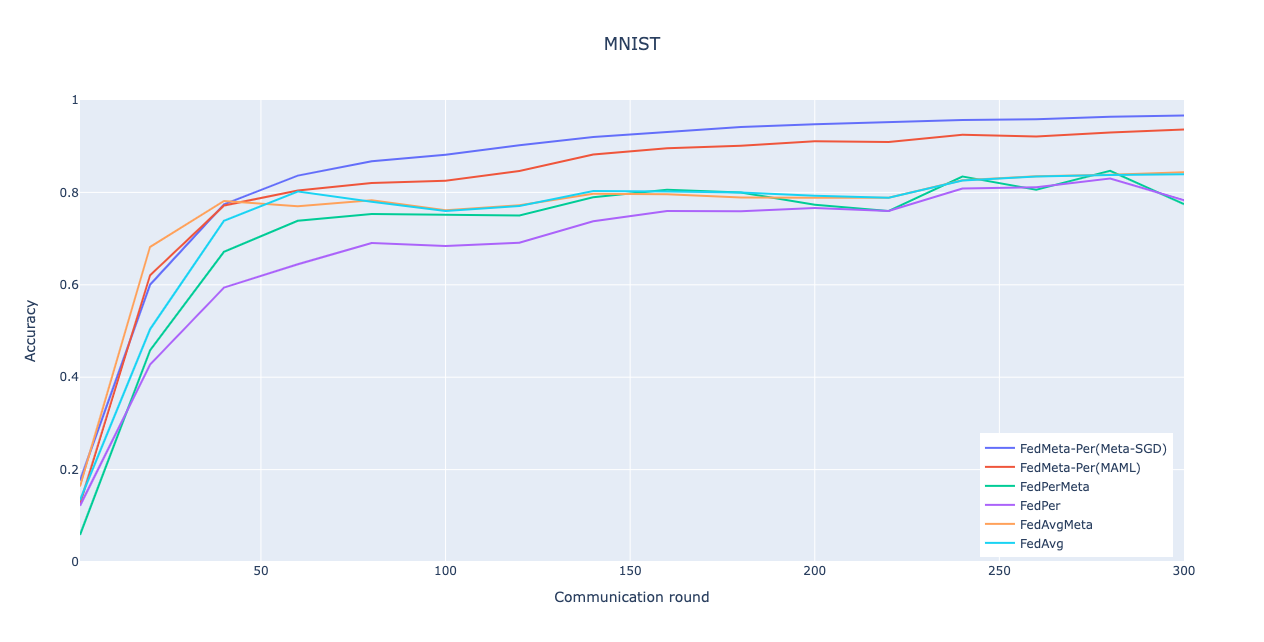
\includegraphics[width=\linewidth]{./tab_img/mnist_per_new.png}
            \caption{MNIST, new clients}
            \label{fig:mnist_per_new}
        \end{subfigure}%
        \begin{subfigure}{.5\textwidth}
            \centering
            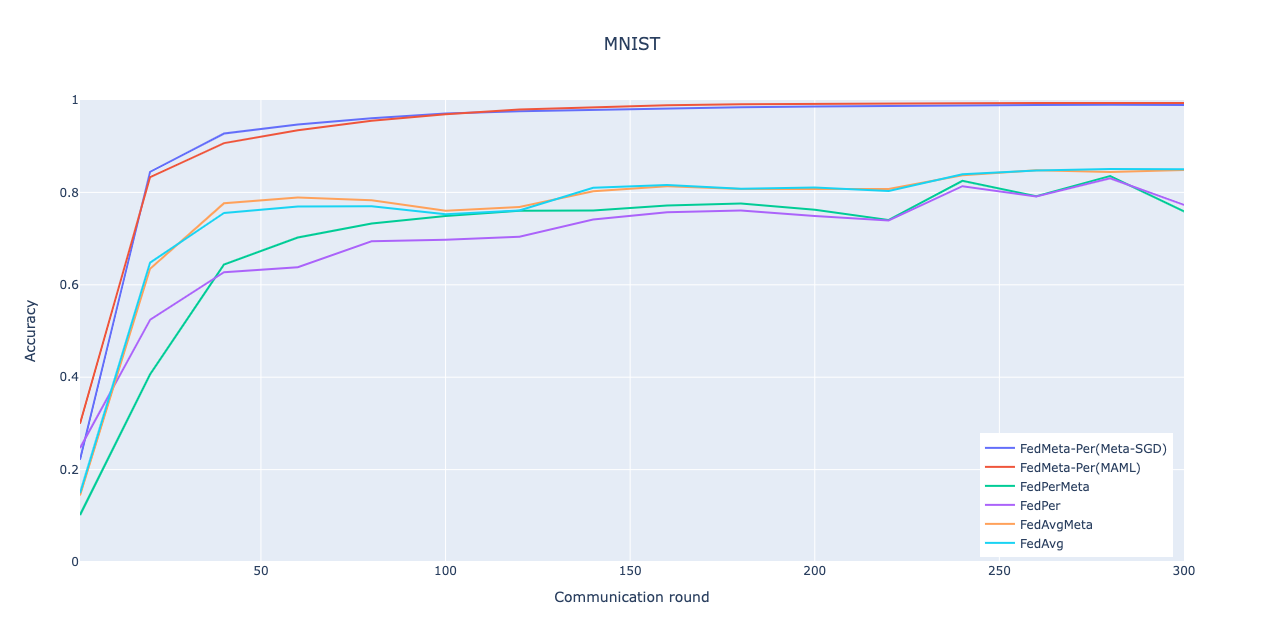
\includegraphics[width=\linewidth]{./tab_img/mnist_per_old.png}
            \caption{MNIST, local clients}
            \label{fig:mnist_per_old}
        \end{subfigure}
        % \caption{A figure with two subfigures}
        % \label{fig:test}
    \end{subfigure}
    \caption{Quá trình hội tụ của FedPer, FedAvg và FedMeta-Per}
    \label{fig:fedper_acc}
\end{sidewaysfigure}

\begin{sidewaysfigure}
    \centering
    \begin{subfigure}{\textwidth}
        \centering
        \begin{subfigure}{.5\textwidth}
            \centering
            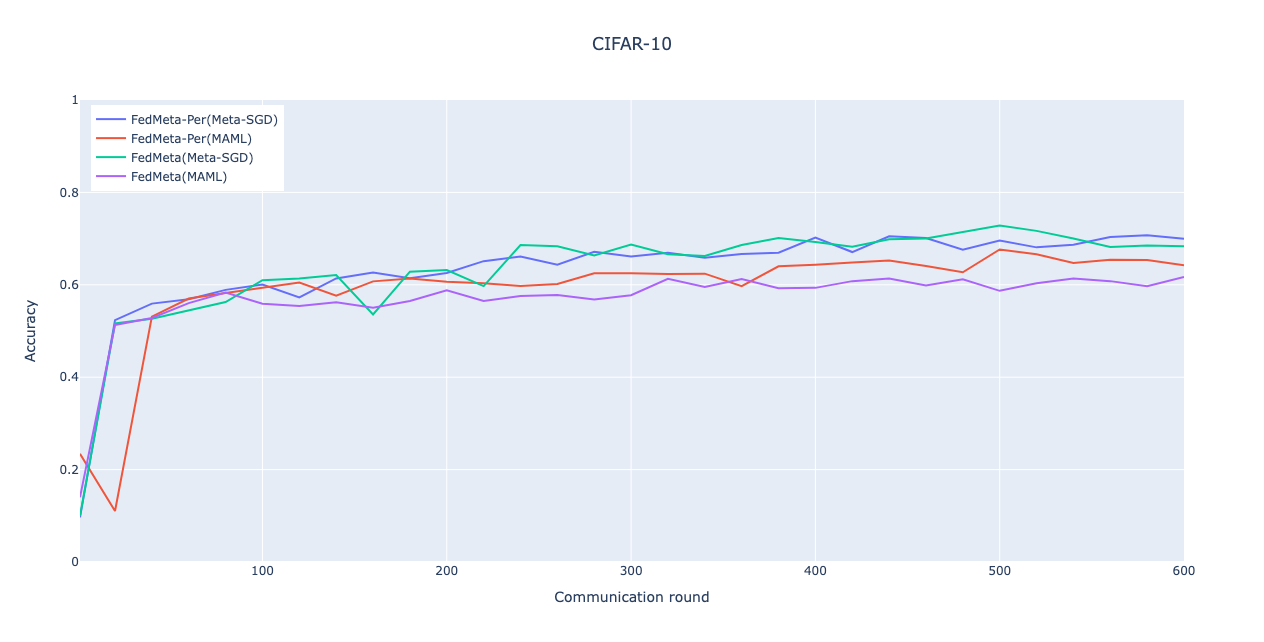
\includegraphics[width=\linewidth]{./tab_img/cifar_meta_new.png}
            \caption{CIFAR-10, new clients}
            \label{fig:cifar_fedmetaper_new}
        \end{subfigure}%
        \begin{subfigure}{.5\textwidth}
            \centering
            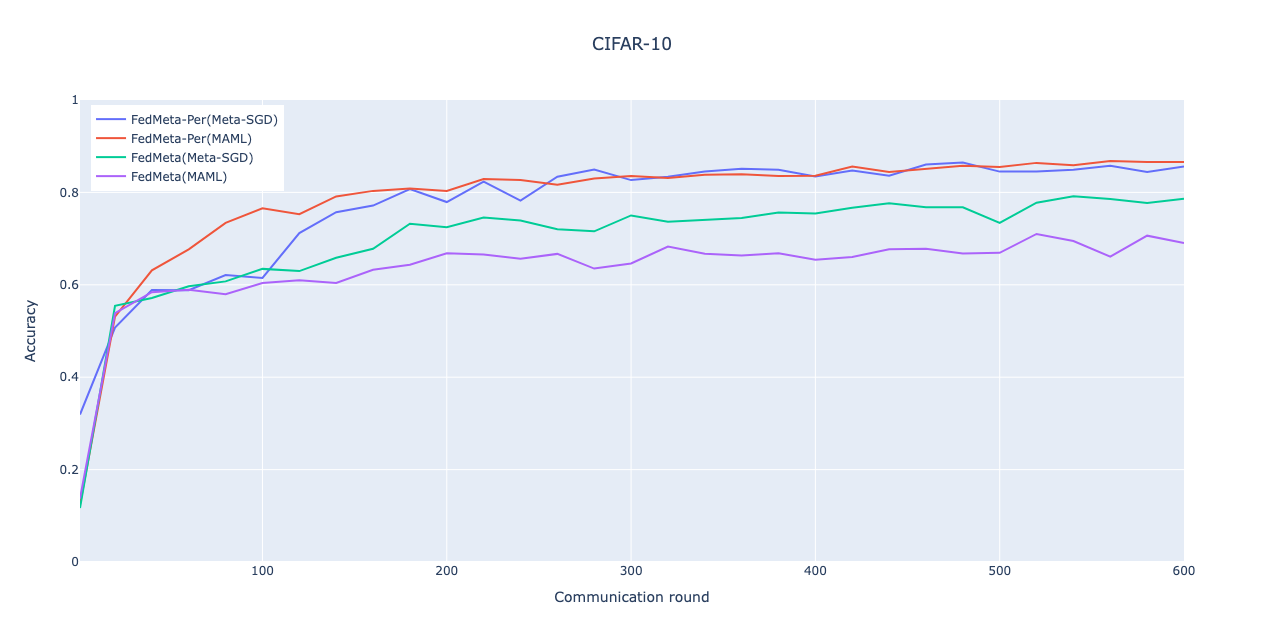
\includegraphics[width=\linewidth]{./tab_img/cifar_meta_old.png}
            \caption{CIFAR-10, local clients}
            \label{fig:cifar_fedmetaper_old}
        \end{subfigure}
        % \caption{A figure with two subfigures}
        % \label{fig:test}
    \end{subfigure}

    \begin{subfigure}{\textwidth}
        \centering
        \begin{subfigure}{.5\textwidth}
            \centering
            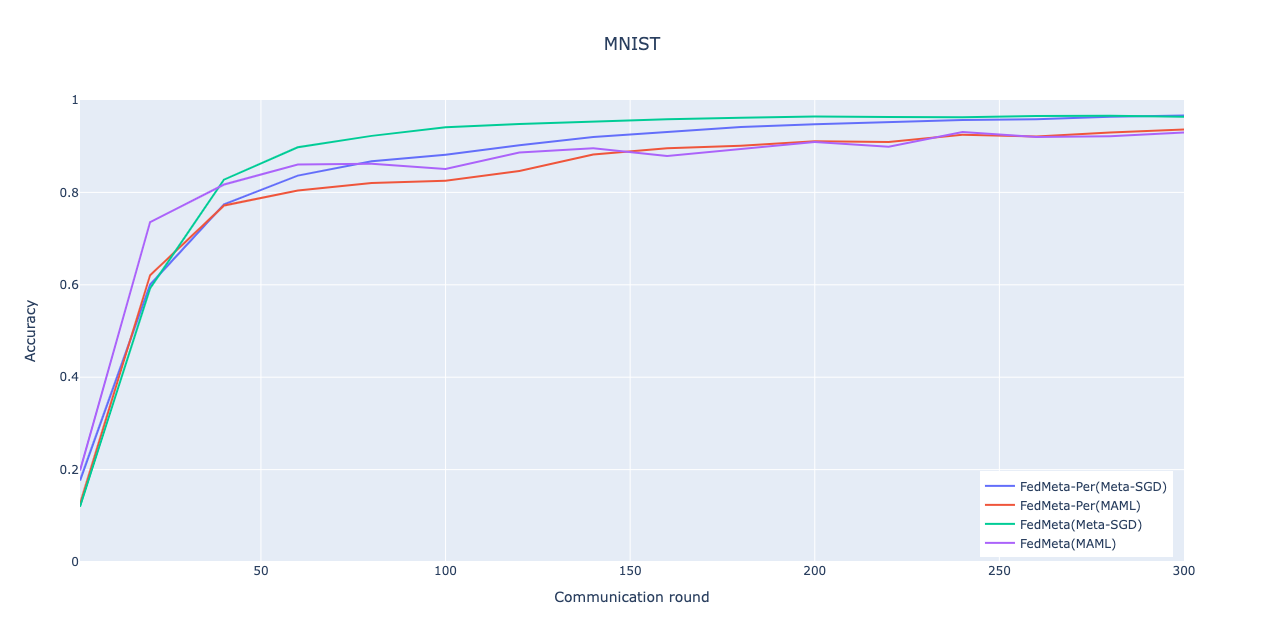
\includegraphics[width=\linewidth]{./tab_img/mnist_meta_new.png}
            \caption{MNIST, new clients}
            \label{fig:mnist_fedmetaper_new}
        \end{subfigure}%
        \begin{subfigure}{.5\textwidth}
            \centering
            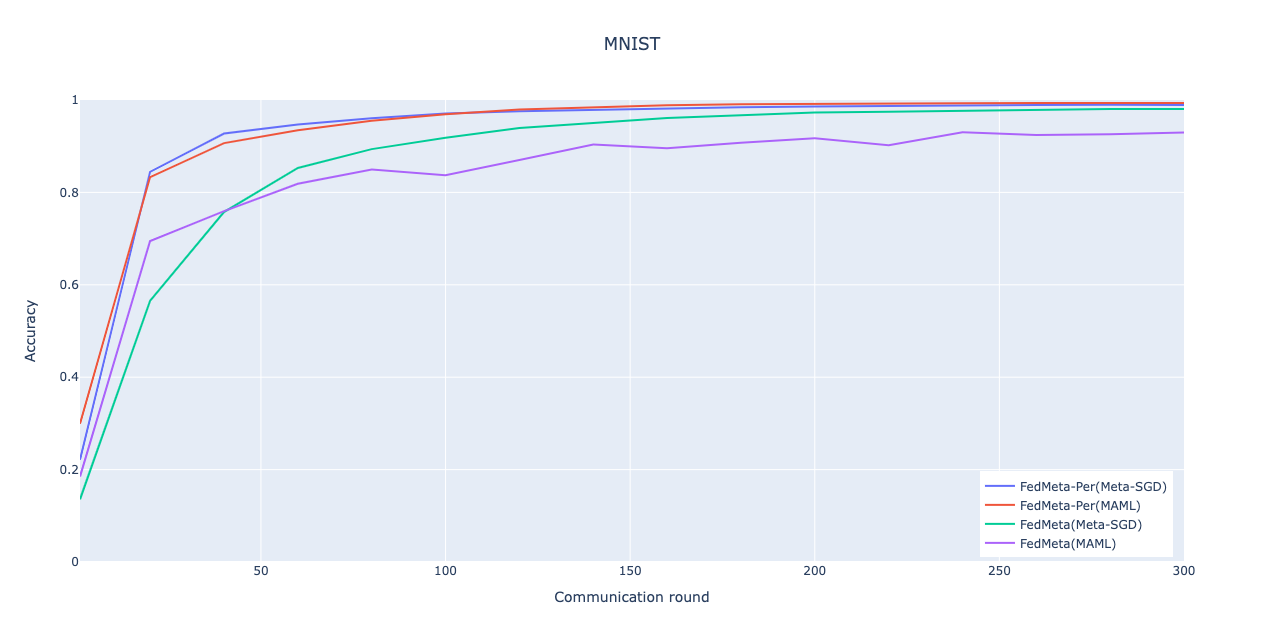
\includegraphics[width=\linewidth]{./tab_img/mnist_meta_old.png}
            \caption{MNIST, local clients}
            \label{fig:mnist_fedmetaper_old}
        \end{subfigure}
        % \caption{A figure with two subfigures}
        % \label{fig:test}
    \end{subfigure}
    \caption{Quá trình hội tụ của FedMeta và FedMeta-Per}
    \label{fig:fedmetaper_acc}
\end{sidewaysfigure}

\section{Phân tích tính cá nhân hoá}

Từ Bảng \ref{tab:mnist} và \ref{tab:cifar}, có thể thấy tính cá nhân hoá của hệ thống FL đã được cải thiện rất nhiều lần nhờ vào việc huấn luyện theo các thuật toán ML. Thật vậy, các kết quả tính trên trung bình của máy khách thu được bởi các thuật toán \codeword{FedMeta} đều có giá trị trung bình lớn hơn và độ lệch chuẩn nhỏ hơn trên hầu hết các thang đo so với \codeword{FedAvg} và \codeword{FedAvgMeta}. Khả năng này đến từ việc fine-tune mộ hình toàn cục (có khả năng thích ứng nhanh trên tập dữ liệu mới) trên tập support của máy khách trong quá trình kiểm thử.

Tuy nhiên, mức cá nhân hoá này thực sự vẫn khá thấp so với kết quả đạt được của hệ thống FL có sử dụng các kỹ thuật PL xét trên độ lệch chuẩn (Bảng \ref{tab:acc_paper}). Trong khi đó, các thuật toán PL không thực hiện fine-tune mô hình của mình trên tập dữ liệu kiểm thử. Việc này chứng tỏ hai điều: \textbf{(1) - Khả năng cá nhân hóa của các thuật toán PL đến từ các lớp phần riêng được đặt tại máy khách, (2) - Việc duy trì các lớp phần riêng trên máy khách cho khả năng cá nhân hóa cao hơn việc fine-tune mô hình toàn cục trên tập support}. Trong thuật toán đề xuất, khoá luận vừa cho phép mô hình toàn cục tinh chỉnh trên tập dữ liệu support của máy khách trước khi kiểm thử, vừa duy trì các lớp phần riêng của mạng học sâu trên các máy khách. Việc này được kỳ vọng giúp làm tăng tính cá nhân hóa hơn nữa cho hệ thống FL. Tính cá nhân hoá của thuật toán đề xuất sẽ được so sánh với các thuật toán \codeword{FedMeta} (vì \codeword{FedPer} và \codeword{FedPerMeta} không hội tụ).

Giá trị của các thang đánh giá giữa \codeword{FedMeta} và \codeword{FedMeta-Per} được trình bày trong Bảng \ref{tab:cifar_} và \ref{tab:mnist_}. Theo đó, thuật toán đề xuất cho kết quả vượt trội hơn từ 3\% đến 25\% so với \codeword{FedMeta} trong hầu hết mọi thang đánh giá (trừ precision trên người dùng mới của CIFAR-10). Xét trên loại người dùng tham gia kiểm thử, đối với người dùng cục bộ, các thang đo có sự chênh lệch rất lớn giữa hai nhóm thuật toán. Cụ thể, các thuật toán \codeword{FedMeta-Per} cho độ chính xác cũng như chất tượng phân lớp tốt hơn rất nhiều so với \codeword{FedMeta}. Nguyên nhân là do tính cá nhân hoá tại từng máy khách được đẩy lên rất cao nhờ vào việc duy trì một phần mạng neuron qua nhiều bước huấn luyện toàn cục. Cũng chính nhờ nguyên nhân này, quá trình hội tụ của \codeword{FedMeta-Per} trên người dùng cục bộ xảy ra nhanh hơn so với \codeword{FedMeta} (Hình \ref{fig:fedmetaper_acc}). Đối với người dùng mới, mặc dù kết quả kiểm thử cuối cho các giá trị tốt hơn khi so sánh thuật toán đề xuất với \codeword{FedMeta}, quá trình hội tụ chưa thực sự ấn tượng. Cụ thể, độ chính xác thể hiện trong hình \ref{fig:cifar_fedmetaper_new} và \ref{fig:mnist_fedmetaper_new} cho thấy sự đồng đều về khả năng hội tụ giữa \codeword{FedMeta} và \codeword{FedMeta-Per}. Tuy nhiên, theo thời gian, khi người dùng mới tham gia vào một hoặc một vài bước huấn luyện toàn cục, độ chính xác cùng chất lượng phân lớp sẽ được tăng lên đến mức bằng với các độ đo thu được trên người dùng cục bộ.

\begin{table}[H]
    \centering
    \caption{Bảng kết quả (\%) của thuật toán FedMeta và FedMeta-Per trên tập dữ liệu CIFAR-10}
    \label{tab:cifar_}
    \resizebox{\linewidth}{!}{%
    \begin{tabular}{c|l|ccccc} 
    \toprule
    \multicolumn{1}{l}{}                             & \multicolumn{1}{c|}{}                   & $acc_{micro}$   & $acc_{macro}$        & $P_{macro}$         & $R_{macro}$          & $F1_{macro}$         \\ 
    \hline
    \multirow{4}{*}{local client}                    & FedMeta(MAML)                           & 69.02          & 68.76±14.86          & 67.42±21.16         & 66.56±13.48          & 61.14±20              \\
                                                     & FedMeta(Meta-SGD)                       & 78.63          & 78.73±11.59          & 74.65±21.12         & 75.25±14.09          & 72.87±18.31           \\
                                                     & \textbf{FedMeta-Per(MAML)}              & \textbf{86.6}  & \textbf{86.52±6.31}  & \textbf{86.43±5.88} & \textbf{85.47±6.87}  & \textbf{85.33±6.77}   \\
                                                     & \textbf{FedMeta-Per(Meta-SGD)}          & 85.61          & 85.68±7.22           & 86.26±6.35          & 85.36±6.83           & 85.08±7.32            \\ 
    \hline
    \multicolumn{1}{l|}{\multirow{4}{*}{new client}} & FedMeta(MAML)                           & 61.69          & 61.64±12.49          & 52.66±26.06         & 59.94±12.35          & 50.76±19.2            \\
    \multicolumn{1}{l|}{}                            & FedMeta(Meta-SGD)                       & 68.36          & 67.89±15.11          & \textbf{70.3±22.37} & 66.86±15.02          & 60.24±21.52           \\
    \multicolumn{1}{l|}{}                            & \textbf{\textbf{FedMeta-Per(MAML)}}     & 64.22          & 63.70±12.29          & 57.06±24.99         & 61.63±12.66          & 53.68±19.06           \\
    \multicolumn{1}{l|}{}                            & \textbf{\textbf{FedMeta-Per(Meta-SGD)}} & \textbf{69.97} & \textbf{69.13±14.63} & 66.53±24.91         & \textbf{67.82±15.34} & \textbf{62.42±20.94}  \\
    \bottomrule
    \end{tabular}
    }
\end{table}

\begin{table}[H]
    \centering
    \caption{Bảng kết quả (\%) của thuật toán FedMeta và FedMeta-Per trên tập dữ liệu MNIST}
    \label{tab:mnist_}
    \resizebox{\linewidth}{!}{%
    \begin{tabular}{c|l|ccccc} 
    \toprule
    \multicolumn{1}{l}{}                             & \multicolumn{1}{c|}{}                   & $acc_{micro}$   & $acc_{macro}$        & $P_{macro}$         & $R_{macro}$          & $F1_{macro}$         \\ 
    \hline
    \multirow{4}{*}{local client}                    & FedMeta(MAML)                           & 92.99           & 91.14±5.99           & 90.56±6.24          & 90.98±5.9            & 90.16±6.28           \\
                                                     & FedMeta(Meta-SGD)                       & 98.02           & 96.35±4.62           & 96.49±4.1           & 95.64±5.94           & 95.80±5.51           \\
                                                     & \textbf{FedMeta-Per(MAML)}              & \textbf{99.37 } & \textbf{99.12±1.29 } & \textbf{99.11±1.3 } & \textbf{98.82±1.99 } & \textbf{98.94±1.6}   \\
                                                     & \textbf{FedMeta-Per(Meta-SGD)}          & 98.92           & 98.15±3.32           & 98.42±1.95          & 98.42±1.96           & 98.20±2.94           \\ 
    \hline
    \multicolumn{1}{l|}{\multirow{4}{*}{new client}} & FedMeta(MAML)                           & 92.96           & 91.88±5.88           & 90.14±7.97          & 90.74±5.95           & 90.02±7.34           \\
    \multicolumn{1}{l|}{}                            & FedMeta(Meta-SGD)                       & 96.39           & 93.53±8.39           & 93.73±10.26         & 88.65±14.06          & 89.31±14.56          \\
    \multicolumn{1}{l|}{}                            & \textbf{\textbf{FedMeta-Per(MAML)}}     & 93.6            & 93.57±5.58           & 93.64±5.56          & 90.98±6.98           & 91.83±6.43           \\
    \multicolumn{1}{l|}{}                            & \textbf{\textbf{FedMeta-Per(Meta-SGD)}} & \textbf{96.62}  & \textbf{95.88±3.58}  & \textbf{95.73±4.11} & \textbf{94.34±5.05}  & \textbf{94.85±4.61}  \\
    \bottomrule
    \end{tabular}
    }
\end{table}

Như vậy, có thể kết luận rằng, \textbf{tính cá nhân hóa của thuật toán đề xuất đã được cải thiện so với các thuật toán trong phần so sánh nhờ vào việc duy trì các lớp phần riêng tại máy khách và việc mô hình tại máy khách thực hiện fine-tune trên tập dữ liệu support trước khi tiến hành kiểm thử}.
